%\documentclass{article}
\documentclass[a4paper,10pt]{article}
\usepackage[utf8]{inputenc}
\usepackage{graphicx}
\usepackage{url}
\usepackage{float}
\usepackage{times}
\usepackage{multirow}
\usepackage{listings}
\usepackage{times}
\usepackage{paralist}
\usepackage{epsfig}
\usepackage{subfigure}
\usepackage[hypertex]{hyperref}
\usepackage{subfigure}
\usepackage{color}

%\documentclass{rspublic}

\usepackage{ifpdf}

\newcommand{\I}[1]{\textit{#1}}
\newcommand{\B}[1]{\textbf{#1}}
\newcommand{\BI}[1]{\textbf{\textit{#1}}}
\newcommand{\T}[1]{\texttt{#1}}

\setlength\topmargin{0in}
\setlength\headheight{0in}
\setlength\headsep{0in}
\setlength\textheight{9in}
\setlength\textwidth{6.5in}
\setlength\oddsidemargin{0in}
\setlength\evensidemargin{0in}
\setlength\parindent{0.1in}
\setlength\parskip{0.25em}


\ifpdf
 \DeclareGraphicsExtensions{.pdf, .jpg}
\else
 \DeclareGraphicsExtensions{.eps, .ps}
\fi

\newcommand{\jha}[1]{ {\textcolor{red} { ***Jha: #1 }}}

\begin{document}

\title{\large The Simple API for Grid Applications: Supporting
  e-Science by Providing Simple, Stable and Generic Programming
  Interfaces}

\author{Joao Abecasis$^{1}$, Shantenu Jha$^{1,2,3}$, Hartmut Kaiser$^{1}$, \\ Andre Merzky$^{1}$, Ole Weidner$^{1}$ \\
  \small{\emph{$^{1}$Center for Computation \& Technology, Louisiana State University, USA}}\\
  \small{\emph{$^{2}$Department of Computer Science, Louisiana State
      University, USA}}\\
  \small{\emph{$^{3}$e-Science Institute, University of Edinburgh, UK}}}

\maketitle

\begin{figure}
\begin{center}
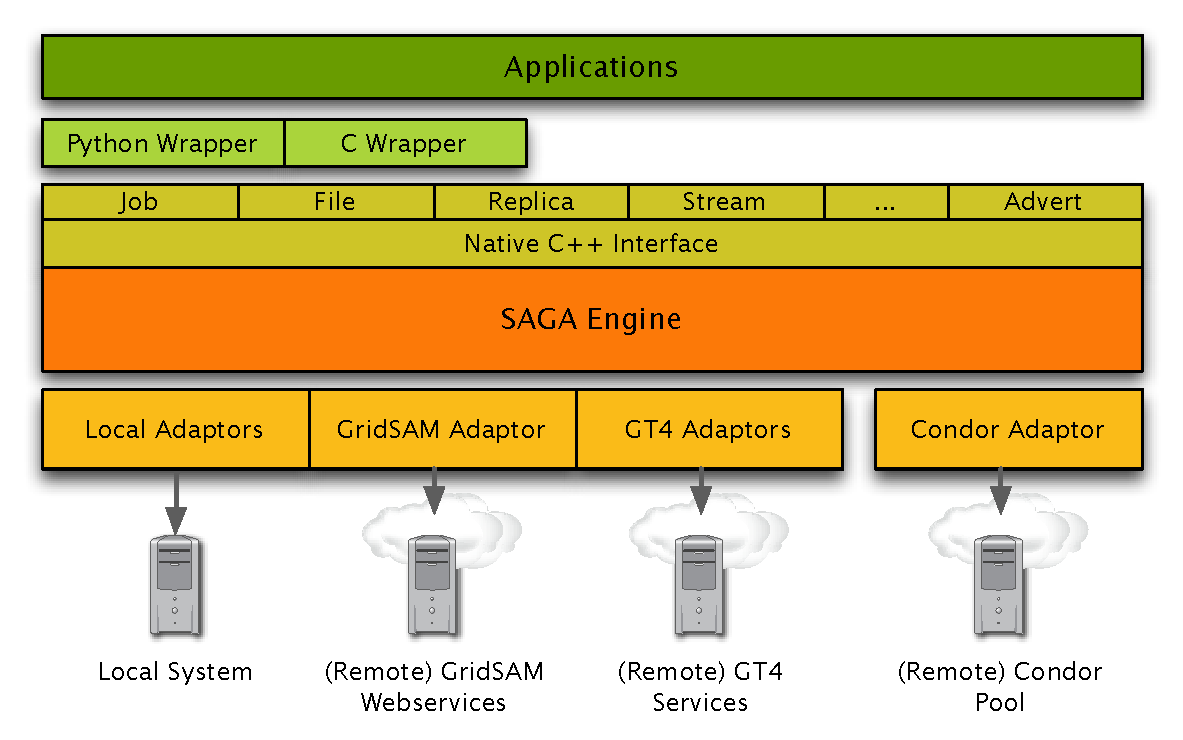
\includegraphics[scale=0.60]{saga_layer_arch}
\end{center}
\caption{A layered diagram of how a typical application uses the C++ SAGA implementation (possibly via the C or Python wrappers) to implement the most commonly  required functionality in distributed environments. The adaptors enable SAGA to be used to different middleware distributions; adaptors are typically loaded run-time and thus enable applications to be written once, but deployable on any system for
which the SAGA adaptors exist.}
\label{fig:saga_arch}
\end{figure}

SAGA is a high level API that provides a simple, standard and uniform
interface to the most commonly required distributed functionality (see
Figure 1).  As shown in Figure 2, SAGA can be used for Grid
applications~\cite{saga_escience07, saga_tg08}, tool-kits that manage
distributed applications, as well as implement abstractions that
support commonly occurring programming, access and usage
patterns~\cite{saga_mapreduce}.  SAGA is currently an OGF approved
technical specification~\cite{saga_gfd90}, on the road map to becoming
a standard.  Although the process that has lead to the SAGA
specification is community driven, the effort to validate, develop a
specification-compliant implementation and to provide effective
adaptors to make SAGA usable on different middleware and distributed
systems has received a major boost by OMII-UK's decision to support
the SAGA effort.

\begin{figure}
\begin{center}
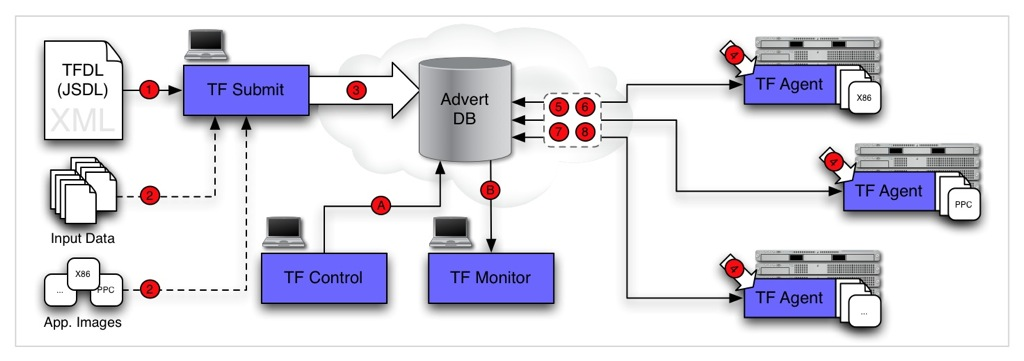
\includegraphics[scale=0.60]{bigpicture_shrimpFarm.jpg}
\end{center}
\caption{A schematic representation of how SAGA can be used to
  orchestrate the distributed resources and provide the required
  functionality. In this case SAGA is used to control the many stages
  of a task-farming application -- a very simple, single stage
  workflow.}
\label{fig:saga_arch}
\end{figure}

The aim of this paper is to provide a brief introduction to SAGA and show
how it is an effective tool for developing e-Science applications.  We
will briefly discuss the sophisticated software development
environments and tools that are used by the SAGA team and which are
necessary, in order to provide simple, stable and usable
implementations of SAGA.  Finally, we will provide a summary and a
roadmap of the many SAGA activities that are being undertaken by the
SAGA team centered out of the Center for Computation and Technology
(CCT) at Louisiana State University (LSU) as part of the OMIISAGA
project\footnote{http://saga.cct.lsu.edu}.  In particular, we will
show how, OMIISAGA in conjunction with other funded projects, for
example, a project to develop Condor adaptors, which will bring SAGA
to Campus Grids and many other high-throughput systems, is making an
impact at every level of the software landscape required for
distributed system -- starting from the application level and
downwards.

\bibliographystyle{IEEEtran} 
\bibliography{saga}


\end{document}

